\chapter{Experiments and Results}

\begin{table*}[!h]
    \centering
    \resizebox{\textwidth}{!}{
        \begin{tabular}{c|c|c|c|c}
            \textbf{Experiment} & \textbf{Avg. PPL} & \textbf{Increase in PPL} & \textbf{Avg. Runtime}   & \textbf{Decrease in Runtime} \\ \hline
            \textit{Baseline}   & \textit{12.6439}  & \textit{0.00\%}          & \textit{0.6476}         & \textit{0.00\%}              \\ \hline
            1 layer - first     & 23508589055.1685  & 185928312366.07\%        & \multirow{3}{*}{0.5611} & \multirow{3}{*}{-13.36\%}    \\
            1 layer - middle    & 13.2905           & 5.11\%                   &                         &                              \\
            1 layer - last      & 22.6169           & 78.88\%                  &                         &                              \\ \hline
            2 layer - first     & 2361030.4434      & 18673177.46\%            & \multirow{3}{*}{0.5449} & \multirow{3}{*}{-15.85\%}    \\
            2 layer - middle    & 13.8172           & 9.28\%                   &                         &                              \\
            2 layer - last      & 23.6517           & 87.06\%                  &                         &                              \\ \hline
            4 layer - first     & 17938.6214        & 141775.70\%              & \multirow{3}{*}{0.5097} & \multirow{3}{*}{-21.30\%}    \\
            4 layer - middle    & 16.6120           & 31.38\%                  &                         &                              \\
            4 layer - last      & 29.4387           & 132.83\%                 &                         &                              \\ \hline
            8 layer - first     & 4740882052.1188   & 37495410512.80\%         & \multirow{3}{*}{0.4388} & \multirow{3}{*}{-32.25\%}    \\
            8 layer - middle    & 28.1565           & 122.69\%                 &                         &                              \\
            8 layer - last      & 52.1473           & 312.43\%                 &                         &                              \\ \hline
            \end{tabular}
    }
    \caption{Results of Experiments}
    \label{tab:results}
\end{table*}

The experiments are conducted first by using the original PhoGPT-4B-Chat model as the baseline model. With 24 Transformer blocks or layers, each with 24 attention heads, the model results in roughly 3.7B parameters.  \par
The model is then modified in multiple ways to reduce the model size by removing different numbers and positions of layers from the model. We had experimented with removing 1, 2, 4, 8 layers consecutively, repeating from the first layer to the last layer possible of the model. The modified model are then evaluated using the perplexity metric on the test prompt dataset. The average perplexity is calculated as metrics to evaluate the performance of the model. \par
The experiments are conducted on a single NVIDIA RTX 3090Ti GPU with 24GB of VRAM, given the following results in Table \ref{tab:results}. \par


As can be seen from the table, the baseline model PhoGPT-4B-Chat has a perplexity of 12.6439 on the test dataset. When removing 1 layer from the model, the perplexity increases to 13.2905 (about 5\%) as average, to tremendously large when removing the critical layers. The results pattern continues as more layers are removed from the model. The perplexity increases as the number of layers removed increases, the first and last layers have much more significant impact on the model's performance compared to the middle layers. \par
The runtime or inference speed of the model is also measured during the experiments. The runtime of the model is measured by calculating the average time taken to generate the output sequences for the test dataset. As the model size decreases, the runtime of the model also decreases. The runtime of the model is inversely proportional to the model size, as the trade-off between model size or performance and inference speed is a common problem in the battlefield of LLMs. \par

\begin{figure*}[!h]
    \centering
    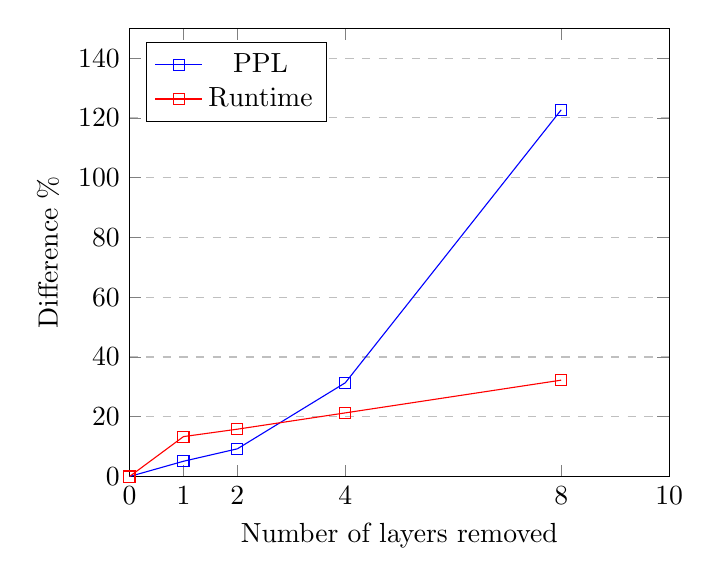
\begin{tikzpicture}
        \begin{axis}[
            title={},
            xlabel={Number of layers removed},
            ylabel={Difference \%},
            xmin=0, xmax=10,
            ymin=0, ymax=150,
            xtick={0,1,2,4,8,10},
            ytick={0,20,40,60,80,100,120,140},
            legend pos=north west,
            ymajorgrids=true,
            grid style=dashed,
        ]
        
        \addplot[
            color=blue,
            mark=square,
            ]
            coordinates {
            (0,0)(1,5.11)(2,9.28)(4,31.38)(8,122.69)
            };
        \addplot[
            color=red,
            mark=square,
            ]
            coordinates {
            (0,0)(1,13.36)(2,15.85)(4,21.30)(8,32.25)
            };
        \legend{PPL,Runtime}
        \end{axis}
    \end{tikzpicture}
    \caption{Model's Perplexity and Runtime results with layers removed}
    \label{fig:results_plot}
\end{figure*}